% File: img/raspberry-pi-computing-cluster.tex
% Compile with
%
%   pdflatex raspberry-pi-computing-cluster.tex
%
\documentclass[tikz]{standalone}
\usepackage{amsmath, inconsolata}
\usetikzlibrary {arrows.meta} 

\begin{document}
    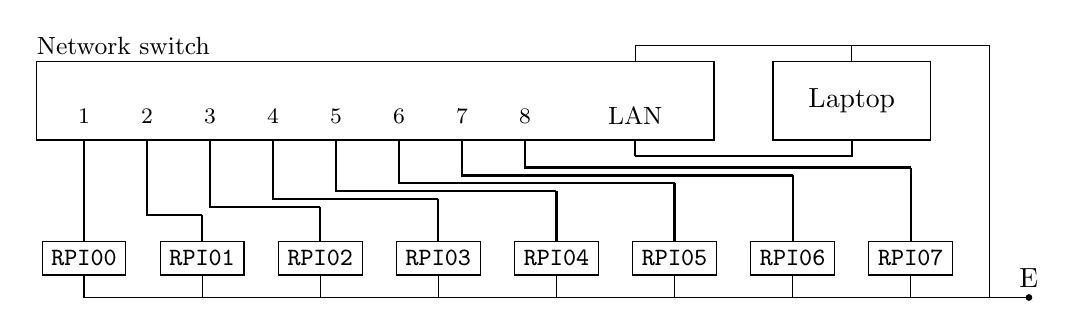
\begin{tikzpicture}[yscale = -1]
        \draw [fill = white] ( -0.6,  0.0) rectangle ( 8.0,  1.0);

        \foreach \i [evaluate = \i as \j using {int(\i+1)}] in {0, ..., 7} {
            \node       (P\i) at (\i * 0.8, 0.7) {\footnotesize{\j}};
            \coordinate (Q\i) at (\i * 0.8, 1.0);
            \coordinate (C\i) at (\i * 1.5, 2.05 - 0.1 * \i);
            \node       (R\i) at (\i * 1.5, 2.5) [draw, fill = white] {\small{\texttt{RPI0\i}}};

            % Ethernet lines
            \draw [thick] (Q\i) |- (C\i.north);
            \draw [thick] (C\i) -- (R\i.north);

            % RPI electricity lines
            \draw (\i * 1.5, 2.7) |- (\i * 1.5 + 1.5, 3.0);
        }

        \node (NStag)  at ( 0.5, -0.2) {\small{Network switch}};
        \node (LANtag) at ( 7.0,  0.7) {\small{LAN}};

        \node [
            draw, fill     = white,
            minimum width  = 20mm,
            minimum height = 10mm
        ] (Laptop) at ( 9.75, 0.5) {Laptop};

        \coordinate (LANcoord1) at (  7.0,  1.0);
        \coordinate (LANcoord2) at (  7.0,  1.2);

        \draw [thick] (LANcoord1)    -- (LANcoord2);
        \draw [thick] (LANcoord2)    -| (Laptop);
        \draw (Laptop.north) -- (9.75, -0.2) -| (11.5,3.0);
        \draw (7.0, -0.0)    |- (9.75,-0.2);

        \filldraw [black] (12.0, 3.0) circle (1pt) node [above] {$\text{E}$};
    \end{tikzpicture}
\end{document}
